\newpage
\section{Amplificador VFA - CFA}
\hspace{1mm} Las especificaciones del VFA LM324 se detallan a continuación.

\begin{itemize}[itemsep=1pt]
    \item $A_{d0}=100~dB$
    \item $f_T=1~MHz$
    \item $f_1=10~Hz$
    \item $f_2=5.06~MHz$
\end{itemize}

\hspace{1mm} Por otro lado, las especificaciones del CFA LM6181 son:

\begin{itemize}[itemsep=1pt]
    \item $R_T=2,37~M\Omega$
    \item $C_T=4,8~pF$
\end{itemize}

\hspace{1mm}   $Z_T $ presenta dos polos en

\begin{itemize}[itemsep=1pt]
    \item $f_1=14~KHz$
    \item $f_2=82,3~MHz$
\end{itemize}

\begin{figure}[!h]
    \centering
    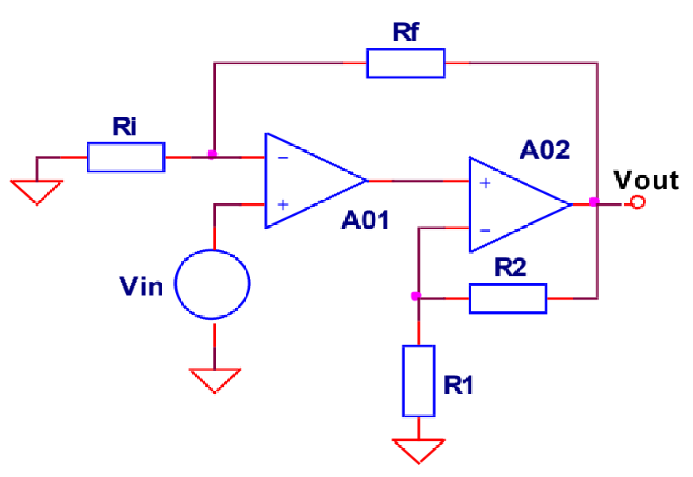
\includegraphics[width=0.7\textwidth]{figuras/11. Lazo cerrado.png}
    \caption{Amplificador compuesto VFA-CFA}
\end{figure}



\subsection{Análisis teórico}
Para el desarrollo de este caso, se considerará que el VFA presenta el mismo comportamiento que el caso anterior. Además, el polo de mayor frecuencia del CFA cuenta con un efecto despreciable sobre la respuesta del amplificador a lazo cerrado.
Con ello, la ecuación del margen de fase para máxima planicidad resulta:

\begin{equation}
    M \varphi = 180^o - arctg \left(\frac{f_g}{f_{1VFA}}\right) - arctg \left(\frac{f_g}{f_{2VFA}}\right) - arctg \left(\frac{f_g}{f_{CFA}}\right) = 65,5^o
\end{equation}

\bigskip
\hspace{1mm} Reemplazando por los valores que son dato.

\begin{equation}
    65,5^o = 180^o - arctg \left(\frac{2~MHz}{10~Hz}\right) - arctg \left(\frac{2~MHz}{5,06~MHz}\right) - arctg \left(\frac{2~MHz}{f_{CFA}}\right)
\end{equation}

\bigskip
\hspace{1mm} Dado que el polo $ f_{1VFA} $ se encuentra lo suficientemente alejado como para no influir sobre la respuesta del amplificador
\begin{equation}
    \Longrightarrow arctg \left(\frac{2~MHz}{10~Hz}\right) = 90^o
\end{equation}

\hspace{1mm} Entonces

\begin{equation}
    65,5^o = 180^o - 90^o - 21,57^o - arctg \left(\frac{2~MHz}{f_{CFA}}\right)
\end{equation}

\bigskip
\hspace{1mm} Resolviendo y despejando se obtiene.

\begin{equation}
    tg (2,93^o) = \frac{2~MHz}{f_{CFA}}
\end{equation}

\bigskip
\hspace{1mm} Entonces, para obtener una máxima planicidad, la frecuencia del polo de lazo cerrado del CFA debe ser

\begin{equation}
    f_{CFA} = \frac{2~MHz}{tg (2,93^o)}
\end{equation}
\begin{equation}
     \boxed{
        f_{CFA} = 39~MHz
    }
\end{equation}

\bigskip
\hspace{1mm} Contando con dicha frecuencia, se procede a calcular la resistencia $ R_2 $ partiendo de la siguiente ecuación:

\begin{equation}
    \omega _{CFA} = \frac{1}{C_T \cdot R_2}
\end{equation}


\begin{align}
   \Longrightarrow R_2 &= \frac{1}{C_T \cdot 2\pi f_{CFA}}
    \\
    R_2 &= \frac{1}{4,8~pF \cdot 2\pi \cdot 39~MHz}
\end{align}

\begin{equation}
    \boxed{
        R_2 = 850~\Omega
    }
\end{equation}

\bigskip
\hspace{1mm} Para calcular la resistencia $ R_1 $ se parte del producto ganancia por ancho de banda.

\begin{equation}
    Avf \cdot f_g = Ado \cdot f_1 \cdot Avf_2
\end{equation}

\bigskip
\hspace{1mm} donde $ Avf_2 $ es la ganancia ideal de lazo cerrado del CFA. Despejando la fórmula anterior

\begin{align}
   \Longrightarrow Avf_2 &= \frac{Avf \cdot f_g}{Ado \cdot f_1} \label{eq:primera} \\
   \nonumber
   \\
         &= \frac{10 \cdot 2~MHz}{100000 \cdot 10~Hz}
\end{align}

\begin{equation}
    \boxed{
    Avf_2 = 20
    }
\end{equation}

\bigskip
\hspace{1mm} Recordando que 

\begin{equation}
    Avf_2 = 1 + \frac{R_2}{R_1} = 20
\end{equation}

\bigskip
\hspace{1mm} Se despeja $ R_1 $ de la ecuación anterior

\begin{align}
   \Longrightarrow R_1 &= \frac{R_2}{Avf_2 - 1} \label{eq:primera} \\
   \nonumber
   \\ 
                       &= \frac{850~\Omega}{20 - 1}
\end{align}

\begin{equation}
    \boxed{
    R_1 = 44,7~\Omega
    }
\end{equation}

\bigskip
\hspace{1mm} Como se plasmó en el marco teórico, al trabajar en máxima planicidad de módulo la frecuencia del polo de la función de transferencia a lazo cerrado se obtiene a partir de la siguiente expresión.

\begin{equation}
    \omega _G = 0,644 \cdot \omega _p 
\end{equation}

\bigskip
\hspace{1mm} Como conducción de diseño, se especifica que el ancho de banda potencial debe ser de $f_G = 2~MHz$. Por lo tanto, reemplazando y despejando $f_p$ de la ecuación anterior 

\begin{equation}
        2\pi \cdot f_G = 0,644 \cdot 2\pi \cdot f_p \\
\end{equation}

\begin{equation}
    \Longrightarrow f_p = \frac{f_G}{0,644} = \frac{2~MHz}{0,644}
\end{equation}

\bigskip
\hspace{1mm} Resultando así.

\begin{equation}
    \boxed{
    f_p = 3,1~MHz
    }
\end{equation}

\bigskip
\hspace{1mm} El ancho de banda a -3dB coincide con la frecuencia del polo a lazo cerrado, que en este contexto específico es de 3.1 MHz. Esta coincidencia surge de la búsqueda de maximizar la planicidad del módulo.




\subsection{Simulaciones}
Nuevamente en este apartado, se simuló el circuito final para evaluar los cálculos obtenidos con anterioridad. El circuito utilizado fue el siguiente:
\begin{figure}[H]
    \centering
    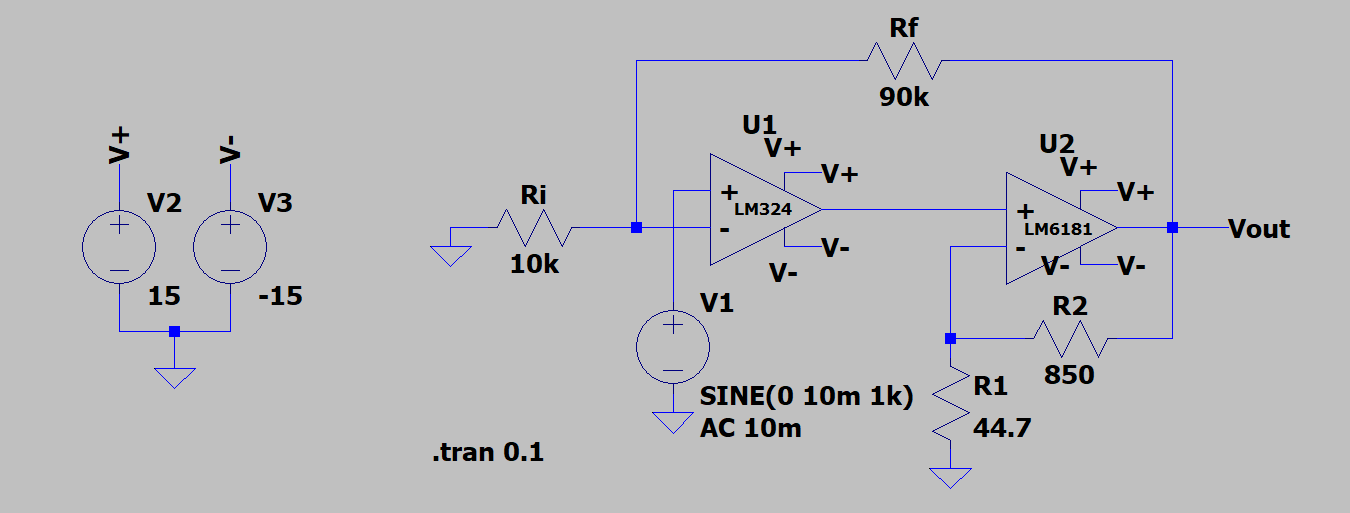
\includegraphics[width=0.9\textwidth]{figuras/Circuito2.png}
    \caption{Circuito VFA - CFA}
\end{figure}


\hspace{1mm} Se comenzó evaluando la ganancia del sistema, para lo cual se graficaron las formas de onda de la entrada y la salida. Con una entrada de $10~mV$, se obtuvo una salida de $97.515~mV$, lo que resulta en una ganancia de:

\begin{figure}[H]
    \centering
    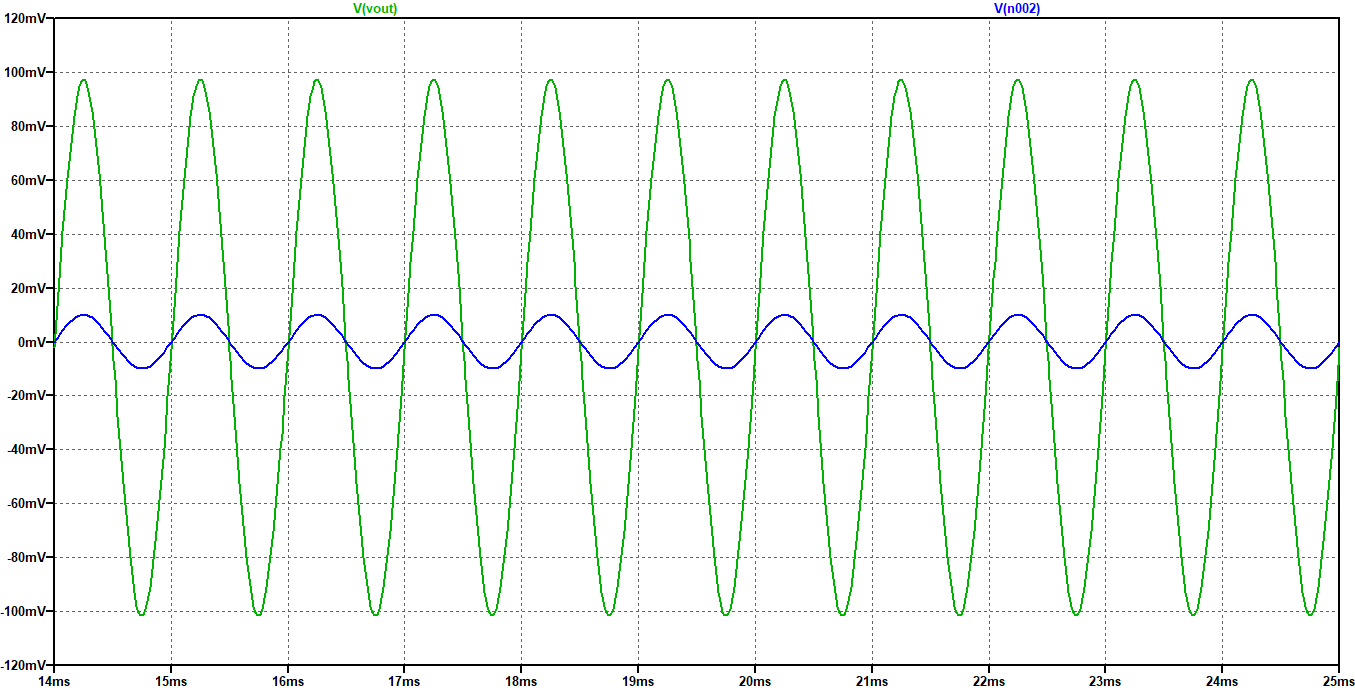
\includegraphics[width=0.9\textwidth]{figuras/Ganancia_c2.png}
    \caption{Ganancia del circuito VFA - CFA}
\end{figure}

\begin{equation*}
    G = \frac{V_{out}}{V_{in}}=\frac{97.515~mV}{10~mv}
\end{equation*}
\begin{equation*}
    \boxed{G = 9.752}
\end{equation*}

\hspace{1mm} Esto implica un error del $2.48\%$ respecto a los cálculos realizados. 

\bigskip
\hspace{1mm}  Posteriormente, se simuló la respuesta en frecuencia del circuito, observándose una ganancia de $20~dB$. La frecuencia de corte, definida por una caída de $-3~dB$, se encuentra en $2.55~MHz$, lo que representa un error de $26.87\%$.

\begin{figure}[H]
    \centering
    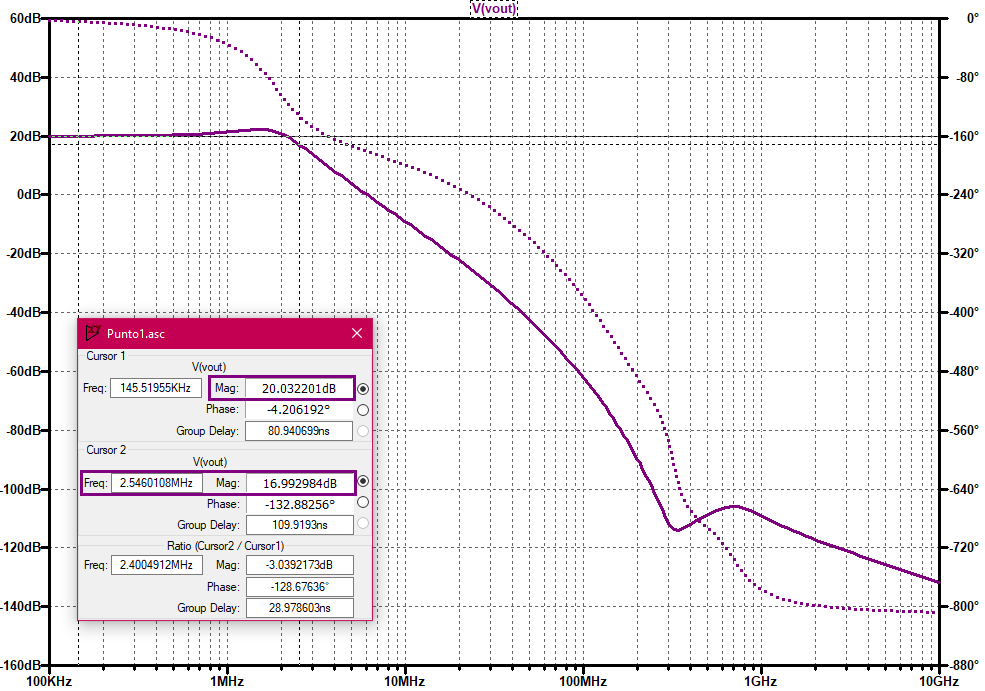
\includegraphics[width=0.9\textwidth]{figuras/Bode_c2.png}
    \caption{Diagrama de Bode del circuito VFA - CFA}
\end{figure}


\subsection{Conclusión}
\hspace{1mm}  En este apartado se diseño un amplificador VFA-CFA, se logró calcular la frecuencia de polo del CFA en $39~MHz$ y las resistencias $R_1$ y $R_2$. Las simulaciones en LTspice mostraron una ganancia de $9.752$ y una frecuencia de corte de $2.55~MHz$, lo que implicó errores de $2.48\%$ y $26.87\%$ respectivamente, en comparación con los cálculos teóricos.

\bigskip
\hspace{1mm}  Comparando ambos amplificadores, el VFA-CFA ofrece una mejor precisión en la ganancia en comparación con el VFA-VFA (error del $7.13\%$) y en la respuesta en frecuencia (error del a $34\%$). Estos resultados subrayan la importancia de seleccionar la topología de amplificación adecuada según las especificaciones del diseño, ya que cada configuración ofrece diferentes niveles de precisión y rendimiento en la simulación y en la práctica.
